\documentclass[dvipdfmx,11pt]{beamer}

% 数式
\usepackage{amsmath,amssymb,bm} %数式環境
\usepackage{mathtools}
\usepackage{physics}
\usepackage{autobreak}

% 画像
\usepackage{graphicx}
\usepackage[dvipdfmx]{color}

% 脚注
\usepackage[hang,small,bf]{caption}

% 括弧
\newcommand{\Bigparen}[1]{\Bigl(#1\Bigr)}
\newcommand{\Bigbrace}[1]{\Bigl\{#1\Bigr\}}
\newcommand{\Bigbrac}[1]{\Bigl[#1\Bigr]}
\newcommand{\Biggparen}[1]{\Biggl(#1\Biggr)}
\newcommand{\Biggbrace}[1]{\Biggl\{#1\Biggr\}}
\newcommand{\Biggbrac}[1]{\Biggl[#1\Biggr]}

\usefonttheme{professionalfonts} %数式フォントをいつも通りにする
\usetheme{metropolis} % Use metropolis theme



\title{}
\author{}
\date{\today}
\institute{所属機関}
\begin{document}
\maketitle

\begin{frame}{目次}
  \tableofcontents
\end{frame}


\section{セクション1}

\begin{frame}

\begin{frame}
  \frametitle{二段組}

  \begin{columns}
    \begin{column}{0.48\textwidth}
        \begin{itemize}
          \item 文字
          \item 表
        \end{itemize}
    \end{column}

    \begin{column}{0.48\textwidth}
        \begin{figure}
          \centering
          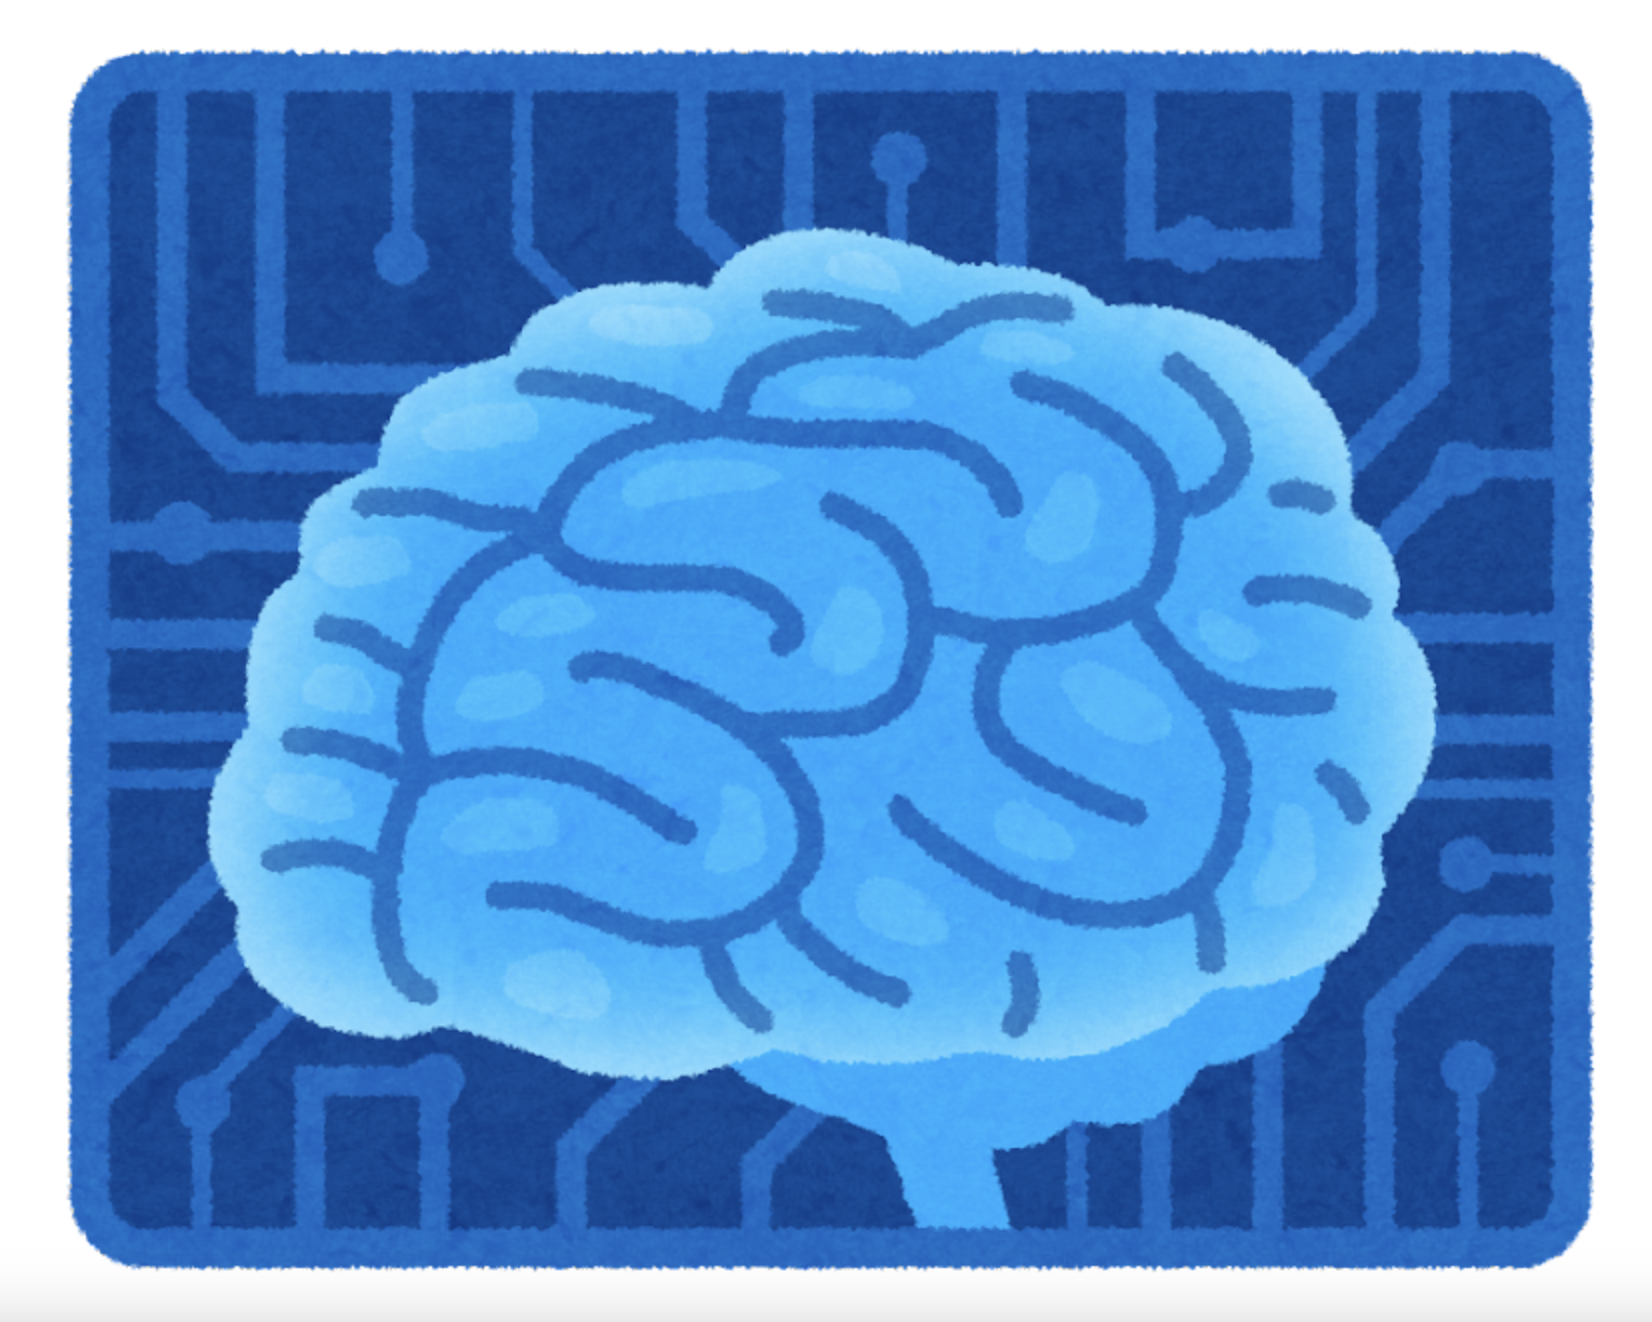
\includegraphics[width=0.8\linewidth]{figure/sample.png}
          \caption{図}
        \end{figure}
    \end{column}
  \end{columns}


\end{frame}





\end{document}




